\documentclass[t, aspectratio=169]{beamer}
\usepackage{amsmath,amsfonts,amsthm,amstext,amssymb, xcolor, tikz, pgf, mathrsfs, polynom, pifont, tabto}

% ----------------------------------------------------------
% Theme Setup

% Use Metropolis Theme
\usetheme[numbering=fraction]{metropolis}
\setbeamertemplate{blocks}[rounded][shadow=false]
\makeatletter
\setlength{\metropolis@titleseparator@linewidth}{1pt}
\makeatother

% Define Colors
\definecolor{chargerblue}{HTML}{002764}
\definecolor{chargerred}{HTML}{e02034}
\definecolor{bggray}{HTML}{d0d3d4}

% Set Colors
\setbeamercolor{title}{fg=chargerblue}
\setbeamercolor{background canvas}{bg=white}
\setbeamercolor{title separator}{fg=chargerred}
\setbeamercolor{structure}{fg=chargerblue}
\setbeamercolor{frametitle}{fg=white, bg=chargerblue}
\setbeamercolor*{normal text}{fg=chargerblue}
\setbeamercolor*{block body}{bg=bggray}
\setbeamercolor*{block title}{bg=chargerblue, fg=white}
% ----------------------------------------------------------

% ----------------------------------------------------------
% Custom Definitions, Commands, Environments, etc.

% Sets of numbers
\def\R{\mathbb{R}} % The reals
\def\N{\mathbb{N}} % The naturals
\def\Z{\mathbb{Z}} % The integers
\def\Q{\mathbb{Q}} % The rationals

% Blank space
\newcommand{\blank}[1]{\underline{\hspace{#1}}} % Blank space

% Change font colors
\newcommand{\cyan}[1]{{\color{cyan}{#1}}} % Changes font to cyan
\newcommand{\red}[1]{{\color{red}{#1}}} % Changes font to red
\newcommand{\magenta}[1]{{\color{magenta}{#1}}} % Changes font to magenta
\newcommand{\orange}[1]{{\color{orange}{#1}}} % Changes font to orange
\newcommand{\yellow}[1]{{\color{yellow}{#1}}} % Changes font to yellow
\newcommand{\violet}[1]{{\color{violet}{#1}}} % Changes font to violet
\newcommand{\green}[1]{{\color{green}{#1}}} % Changes font to green
\newcommand{\blue}[1]{{\color{blue}{#1}}} % Changes font to blue
\newcommand{\white}[1]{{\color{white}{#1}}} % Changes font to white

% Fitted inclusion symbols
\newcommand{\fp}[1]{\left({#1}\right)} % Fitted parentheses around content
\newcommand{\fb}[1]{\left[{#1}\right]} % Fitted brackets
\newcommand{\lhoi}[1]{\left({#1}\right]} % Left half-open interval
\newcommand{\rhoi}[1]{\left[{#1}\right)} % Right half-open interval
\newcommand{\set}[1]{\left\{{#1}\right\}} % Fitted braces (useful for sets)
\newcommand{\av}[1]{\left|{#1}\right|} % Fitted absolute value bars

% Augmented Matrix Environment
\newenvironment{amatrix}[1]{%
	\left[\begin{array}{@{}*{#1}{c}|c@{}}
	}{%
	\end{array}\right]
}

% Miscellaneous
\def\then{\Rightarrow}
\def\to{\rightarrow}
\def\dg{^{\circ}}
\newcommand{\?}{\stackrel{?}{=}}
\newcommand{\cmark}{\text{ \ding{51}}}
\newcommand{\xmark}{\text{ \ding{55}}}

% Coordinate Plane (Four-Quadrant)
\def\coordplane {
	\begin{tikzpicture}        \draw[step=0.25cm,black,very thin,opacity=0.25] (-2.5cm, -2.5cm) grid (2.5cm, 2.5cm);
		\draw[<->,thick,black] (-2.5cm, 0) -- (2.5cm, 0) node[anchor=north west,pos=0.94,font=\scriptsize]{$x$};
		\draw[<->,thick,black] (0,-2.5cm) -- (0, 2.5cm) node[anchor=south east,font=\scriptsize,pos=0.94]{$y$};
	\end{tikzpicture}
}

% Coordinate Plane (One-Quadrant)
\def\onequad {
	\begin{tikzpicture}
		\draw[step=0.25cm, black, very thin, opacity=0.25] (0,0) grid (7.5cm,5cm);
		\draw[->, thick, black] (0,0) -- (7.5cm, 0) node[anchor=north west,font=\scriptsize,pos=0.94]{$x$};
		\draw[->, black, thick] (0,0) -- (0,5cm) node[anchor=south east,font=\scriptsize,pos=0.94]{$y$};
	\end{tikzpicture}
}
% ----------------------------------------------------------

% ----------------------------------------------------------
% Presentation Information
\title[7-2]{Confidence Intervals for the Mean when $\sigma$ is Unknown}
\subtitle{Section 7-2}
\author{Jacob Ayers}
\institute{Lesson \#22}
\date{MAT 110}
% ----------------------------------------------------------

\begin{document}
	
	% Slide 1 (Title Slide)
	\begin{frame}
		\titlepage
	\end{frame}
	
	% Slide 2 (Objectives)
	\begin{frame}{Objectives}
		\begin{itemize}
			\item Construct confidence intervals for $\mu$ when $\sigma$ is not known
		\end{itemize}
	\end{frame}

	\begin{frame}{The $t$ Distribution}
		Last week, we learned how to construct confidence intervals when we knew the population standard deviation $\sigma$. \pause
		
		But more often than not, we don't know $\sigma$. \pause
		
		In this case, we estimate $\sigma$ by using the sample standard deviation $s$. \pause
		
		When we use $s$, we have a little less certainty about our interval estimates. So we need to cast a wider net in order to have the same level of confidence that $\mu$ will be in the interval.
	\end{frame}

	\begin{frame}{The $t$ Distribution}
		To cast this wider net, we use a different probability distribution - the \textit{Student $t$ distribution}, or simply the $t$ distribution. \pause
		
		Like the standard normal distribution we used before, the $t$ distribution has a table. I've posted it in Moodle. \pause
		
		The assumptions used for constructing confidence intervals with the $t$ distribution are the same as those for the standard normal distribution. Namely, \begin{enumerate}[1)]
			\item Sample must be a random sample
			\item Sample size must be 30 or more, or variable is normally distributed if not
		\end{enumerate}
	\end{frame}

	\begin{frame}{The $t$ Distribution}
		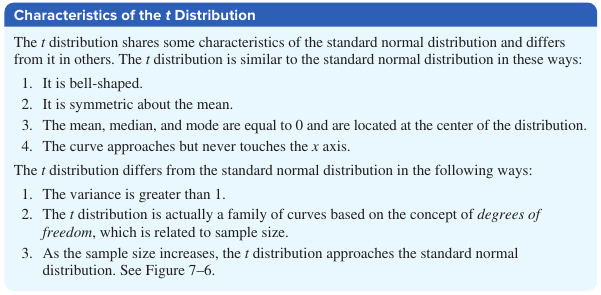
\includegraphics[width=0.75\textwidth]{t-char.png}
	\end{frame}

	\begin{frame}{The $t$ Distribution}
		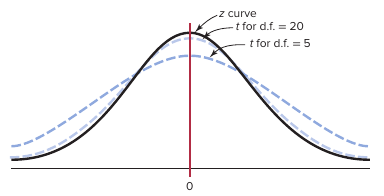
\includegraphics[width=0.75\textwidth]{t-graph.png}
	\end{frame}

	\begin{frame}{Degrees of Freedom}
		A commonly used notion is statistics is that of \textit{degrees of freedom} (d.f.). \pause
		
		The degrees of freedom are the number of values that are free to vary after a sample statistic has been computed. \pause Their purpose is to tell the researcher which curve to use when a distribution is a family of curves (like the $t$ distribution). \pause
		
		Example: Say I know the mean of 5 numbers is 10. \pause \\
		4 of the 5 numbers can be whatever I want them to be (i.e. free to vary). \pause \\
		But once I lock in a set of 4 numbers, the fifth number is also locked in. \pause \\
		This is because I know the 5 numbers have to add up to 50, and there's only one fifth number that'll get me there once I know the values of the other 4. \pause
		
		The $t$ distribution uses $n - 1$ degrees of freedom.
	\end{frame}

	\begin{frame}{Using the $t$ Table to Find $t_{\alpha/2}$}
		Find the $t_{\alpha/2}$ value for a 95\% confidence interval when the sample size is $15$. \pause
		
		Since the sample size is $15$, d.f. = 14. \pause
		
		So looking up 95\% with d.f. = 14, we find that $t_{\alpha/2} = 2.145$ \vspace{1in} \pause
		
		Find the $t_{\alpha/2}$ value for a 99\% confidence interval when the sample size is 23. \pause
		
		Since the sample size is $23$, d.f. = 22. \pause
		
		So looking up 99\% with d.f. = 22, we find that $t_{\alpha/2} = 2.819$
	\end{frame}

	\begin{frame}{Constructing Confidence Intervals}
		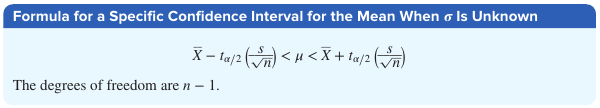
\includegraphics[width=\textwidth]{conf-form.png} \pause
		
		The process for constructing a confidence interval when $\sigma$ is unknown is as follows: \pause \begin{enumerate}[1)]
			\item Make sure the assumptions hold. \pause
			\item Use a calculator to compute $\dfrac{s}{\sqrt{n}}$; store it. \pause
			\item Look up the $t_{\alpha / 2}$ value. \pause
			\item Use the formula above to find your lower/upper limits; write the interval.
		\end{enumerate}
	\end{frame}

	\begin{frame}{Constructing Confidence Intervals}
		A random sample of high temperatures for 12 recent Thanksgiving Days had an average of $42\dg$ F. Assume the variable is normally distributed and the standard deviation of the sample temperatures was $8\dg$ F. Find the 95\% confidence interval of the population mean for the temperatures. \pause
		
		1) The variable is normally distributed; the assumption holds. \pause \\
		2) $\dfrac{s}{\sqrt{n}} = \dfrac{8}{\sqrt{12}} \approx 2.309401077$; store it. \pause \\
		3) Using 95\% and d.f.=11, $t_{\alpha/2} = 2.201$. \pause \\
		
		4) Lower Limit for CI: $42 - 2.201(2.3094) = 36.9\dg$ F \pause \\
		Upper Limit for CI: $42 + 2.201(2.3094) = 47.1\dg$ F \pause
		
		The confidence interval is $36.9\dg\text{ F} < \mu < 47.1\dg\text{ F}$
	\end{frame}

	\begin{frame}{Constructing Confidence Intervals}
		The number of calories per candy bar from a random sample of standard-size candy bars is shown below. Estimate the mean number of calories per candy bar with 98\% confidence. Assume the variable is normally distributed.
		
		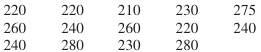
\includegraphics[width=2in]{candy-data.png} \pause
		
		Before we begin, we need to find $\overline{X}$ and $s$. \pause
		
		Using a calculator: $\overline{X} \approx 243.2$; $s \approx 23.8$ \pause
		
		1) Assumptions hold. \pause \\
		2) $\dfrac{s}{\sqrt{n}} = \dfrac{23.8}{\sqrt{14}} \approx 6.360817558$; store it. \pause \\
		3) Using 98\% and d.f.=13, $t_{\alpha/2} = 2.650$.
	\end{frame}

	\begin{frame}{Constructing Confidence Intervals}
		$\overline{X} = 243.2$; $\dfrac{s}{\sqrt{n}} \approx 6.360817558$; $t_{\alpha/2} = 2.650$ \pause
		
		4) Lower Limit for CI: $243.2 - 2.650(6.3608) = 226.3$ \pause \\
		Upper Limt for CI: $243.2 + 2.650(6.3608) = 260.1$ \pause
		
		Confidence Interval: $226.3 < \mu < 260.1$
	\end{frame}

	\begin{frame}{Next Steps}
		\begin{itemize}
			\item Read 7-3
			\item Watch Video Lesson \#23
			\item Prepare for and take Midterm 2 \begin{itemize}
				\item Study Guide posted in Week 13 section
				\item Will take next Wednesday
			\end{itemize}
			\item Complete Assignment 11
		\end{itemize}
	
		\vfill
		
		Thanks for watching!
	\end{frame}
	
\end{document}